\section{Introduction}

The importance of weather forecasting cannot be understated. We regularly
consult weather forecasts to inform our clothing choices, to help us decide
whether a family outing should be a trip to the beach or to a museum; should we
bring along an umbrella? is it shirt-and-shorts weather?\footnote{Incidentally
  it is never \emph{shirt-and-\textbf{short}-shorts weather.}} These are
legitimate concerns, but they are decidedly \emph{first-world} concerns. In
parts of the world where the amount of rainfall literally means life or death it
is plainly obvious that forewarning of drought is of paramount importance.
Whereas wealthy nations may import food and water in times of need, much of
sub-Saharan Africa relies on the prosperity of local agriculture to meet dietary
needs. Any negative impact on the harvest -- here we concern ourselves only with
climatological causes -- will severely restrict available food sources
\citep{development2006mapping}.

Modern Africa has been plagued by socioeconomic struggles, with frequent civil
war, little access to education and medicine, and highly unstable
governments. While much progress has been made in recent years\footnote{For more
  information see \url{https://africaindata.org}} the extra stresses of food
shortages and drought may trigger a return to instability.
% TODO Provide actual citation for above. Is the last line here a
% bit... insensitive?
In 2016 the UN Office for the Coordination of Humanitarian Affairs (UNOCHA)
published a report on the response to \elnino{} in East and Southern Africa
\citep{unocha2016}; by their estimates over 19.5 million people and 10.5
children were affected in East Africa alone. As a result of \elnino{} parts of
East Africa received below average rainfall leading to poor harvests and food
shortages. Similarly, parts of Southern Africa experienced the worst drought for
35 years and leading to huge food insecurity. As one of the worst hit countries,
Kenya alone now has over 1.2 million people in a food security crisis.

Malaria has long been a leading cause of death in Africa, particularly in
children, accounting for approximately 18\% of total deaths in children
\citep{IMHE2016}. \citet{Alles1998} states that, at the time of reporting,
malaria transmission intensities---a measure of how effectively malaria is
transmitted in a population---are often two orders of magnitude greater than other
regions where malaria is a significant problem. \citet{loevinsohn1994}
investigated the relationship between climatic warming and malaria incidence
rates in Rwanda, East Africa. The report found that during the particularly warm
period of the late 1980s malaria incidence rates almost doubled, with even
regions previously free of the disease showing an up-take in
incidence.\footnote{Interestingly, the report notes that while there was no
  significant trend in precipitation over the same period, there was heavy rain
  in the years 1987 and 1988 which coincided with a strong ENSO event.}

More recently \cite{craig2004} sought to quantify the association between
various climatic factors---including rainfall and temperature---and malaria
incidence. The report found that \emph{total seasonal cases} of malaria were not
driven by climatological factors; however there was a strong correlation between
interseasonal variability and factors such as the maximum temperatures of the
preceding season.


% For this reason, it is imperative that we improve our understand of and ability
% to predict this effect in order that we may better prepare and coordinate
% responses to prevent humanitarian disasters.

%% % Would like to say something here referencing data on drought related
%% % deaths in Africa.
%% Indeed forewarning of any impending weather is
%% important for different reasons depending on the local agriculture:
%% forecasting drought allows for stockpiling of water and foods;
%% forecasting of inclement weather allows for farmers to prepare for a
%% greater yield, and locals to prepare for possible flooding.
%% % What other reasons are there for forecasting? This needs rewriting
%% % anyway, as it is a bit ugly in terms of wording. Could be more poetic.
%% Where discussion of the weather is not ``should I wear a raincoat?''
%% but ``will we have enough drinking water?'' weather forecasting should
%% be considered a humanitarian imperative. 
% Is there something to say about global warming here? Probably.

\vspace{1cm}

Early twentieth century observations of atmosphere pressures showed a peculiar
relationship between those measurements in the western tropical Pacific and
those in the southeastern tropical Pacific \citep{holton1989}. Namely, that they
were out of phase --- when one measure was positive, the other was negative.
This was termed the \emph{Southern Oscillation}. Later studies \ref{TODO} would
show that there were accompanying variations in rainfall, sea surface
temperatures, and wind patterns. The combination of these effects would come to
be known collectively as the \elnino{} \emph{Southern Oscillation}, with the
warm phase named \elnino{} and the cold phase \nina{}.


\subsection{Southern Oscillation}
Since the late 19th century, the existence of a large scale `seesaw' in oceanic
surface pressure across the Pacific had been observed \citep{trenberth2000}. The
essence of this observation is that when air pressure is high over the Pacific
Ocean, air pressure tends to be lower over the Indian Ocean (and vice versa)
\citep{philander1990}; from this it was inferred that the two regions were
causally connected by some then-unknown meterological teleconnection. It was
Walker and Bliss who, in the 1930s, characterised this pattern using measures
% Could/should probably say in more detail how exactly they characterised this
such as sea level pressure and precipitation, naming it the Southern Oscillation
(SO). Walker also defined an index for the SO, calling it the Southern
Oscillation Index (SOI). Figure \ref{fig:slp_corr} shows the average spatial
distribution of SOI correlations for the Pacific, showing the eastern and
western Pacific to be out of phase.
% TODO Some more discussion of indices here. Describe exactly what SOI is,
% describe other indices, particularly ones we use.

\begin{figure*}
  \centering
  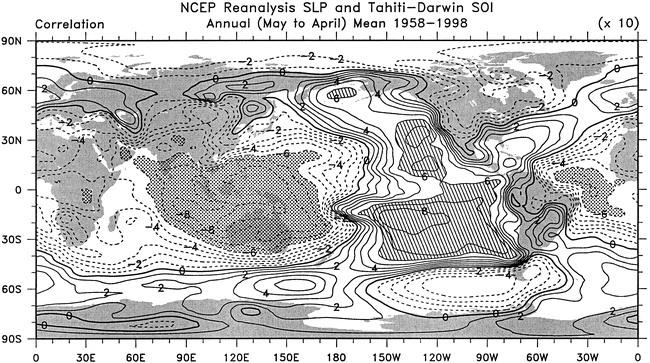
\includegraphics[width=0.75\textwidth]{figures/slp_corr}
  \caption{Sea level pressure correlations with Southern Oscillation Index, a
    measure of the SO devised by Walker. Regions with correlations $>0.6$ are
    hatched and those $<-0.6$ are dotted. It is clear to see that the eastern
    and western tropical Pacific ocean are anticorrelated. Figure taken from
    \cite{trenberth2000}.
    % TODO Is it clear? Maybe this needs more exposition.
  }
  \label{fig:slp_corr}
\end{figure*}

While Walker managed to characterise the atmospheric component of the SO, the
interannual pressure fluctations driving it were irregular and there was not
enough data for Walker to determine whether the ocean was involved in the
system.

\vspace{0.5cm}

In his seminal 1961 study Bjerknes began formulating a model of how the
interaction of both athmospheric and oceanic components could lead to the
appearance of \elnino{} conditions over the tropical Pacific
\citep{bjerknes1961}. He reasoned that much of the connection lied in weakening
of trade (east-to-west equatorial) winds owing to natural fluctuations caused,
for example, by the uneven solar radiation. The trade winds at the sea surface
drag surface water with them. When the trade winds weaken, the friction between
air and sea surface is reduced, thus allowing warmer western Pacific water to
flow to the cooler east. An abundance of warm water along equatorial South
America then surges into the Peruvian coast, as observed by the Peruvian
fishermen.

Later \citep{bjerknes1966} it was also noted that weakening of the trade winds
would lead to reduced upwelling. The general view of the tropical Pacific is of
relatively warmer waters in the west (near Australia), gradually cooling towards
the east (near Peru). This is typically described as having a thermocline (where
cold water meets warm water) gradually rising from west to east. If the trade
winds weaken the thermocline becomes depressed in the east due to the
aforementioned resurgence of warm water. The anomalous warming of seas then
imparts energy into the atmosphere above. Bjerknes states in his conclusion:
``So much seems certain, however, that the extensive warmings of the East
Pacific equatorial waters are due to a weakening of the equatorial easterly
winds to such an extent that (a) the normal upwelling appreciably weakens of
even ceases'', making the case for an ocean-atmosphere connection.

A key result of \citep{bjerknes1966} is that by using the above reasoning
Bjerknes was able to link strengthening of westerlies in the middle latitudes
occuring with accompanying warming of equatorial ocean water. Bjerknes reasoned
that anomalous warming of surface water would then increase the \emph{Hadley
  circulation} rate, thus leading to increased westerly wind strengths.

The Hadley circulation is the poleward atmospheric circulation of
equatorial air away from the equator. The process is diagrammed in
\ref{fig:hadleycell} and is as follows \citep{geomar6557}. Warm air carried by
the trade winds (moving in an easterly and equatorial direction) converges at
the equator where it releases moisture and rises. The Earth's rotation causes a
Coriolis force which results in the rising air being pushed poleward. The
Coriolis force is clockwise in the Northern hemisphere and anti-clockwise in the
Southern hemisphere; in both cases, as the air moves poleward it also
experiences an eastward motion, whereas at the equator it is moving westward
with the trade winds. Having cooled, the air begins to sink at the upper
latitudes, where the Coriolis force now brings the air back towards the equator,
eventually with an easterly component --- the trade winds.

\begin{figure}[t]
  \centering 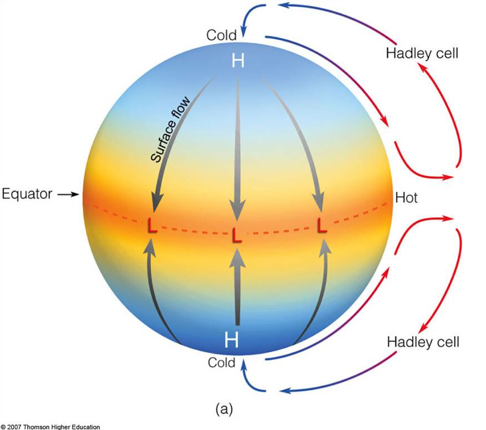
\includegraphics[width=0.9\linewidth]{figures/hadleycell.png}
  \caption{The Hadley circulation. Warm air rises at the equator, is pulled away
    from the equator and towards the poles, cools and falls at greater
    latitudes, then is pulled back towards the equator. This circulation is
    largely created by uneven solar heating and the Coriolis force due to the
    Earth's rotation.}
  \label{fig:hadleycell}
  % From https://www.seas.harvard.edu/climate/eli/research/equable/hadley.html
\end{figure}

Bjerknes continued his investigation into the causes and effects of anomalous
heating in the tropical Pacific ocean and atmospheric pressure variation in his
1969 study \emph{Atmospheric Teleconnections from the Equatorial Pacific}
\citet{bjerknes1969}. In this study a clear connection between \elnino{} and the
SO was demonstrated, particularly that a 1963 \elnino{} event caused a strong
response in the SO.

Figure \ref{fig:pressureprofiles} shows how the dynamic height of a number of
isobars (surfaces of constant atmospheric pressure) varies along the equator
during the months January 1960, and July 1960. In both months it can be seen
that, in the region marking the Pacific ocean, the streamline gradient closest
to the sea surface is towards the west (indicated in \ref{fig:pressureprofiles}
by the line ``S.L.''). Since the streamline gradient shows us how air would move
subject to atmospheric pressure, we can infer that air at that height is moving
east-to-west. As that air moves westward, the sea surface is warming and so the
air warms also, rising as it does. Next we see that at greater heights (in
Figure \ref{fig:pressureprofiles}, lines ``300'' to ``150'', the gradient of the
streamlines is reversed, and we have west-to-east motion along these
streamlines. Progressing eastward and cooling, the air begins to fall,
eventually completing one cycle of what Bjerknes labelled the \emph{Walker
  Circulation}.

\begin{figure}[t]
  \centering
  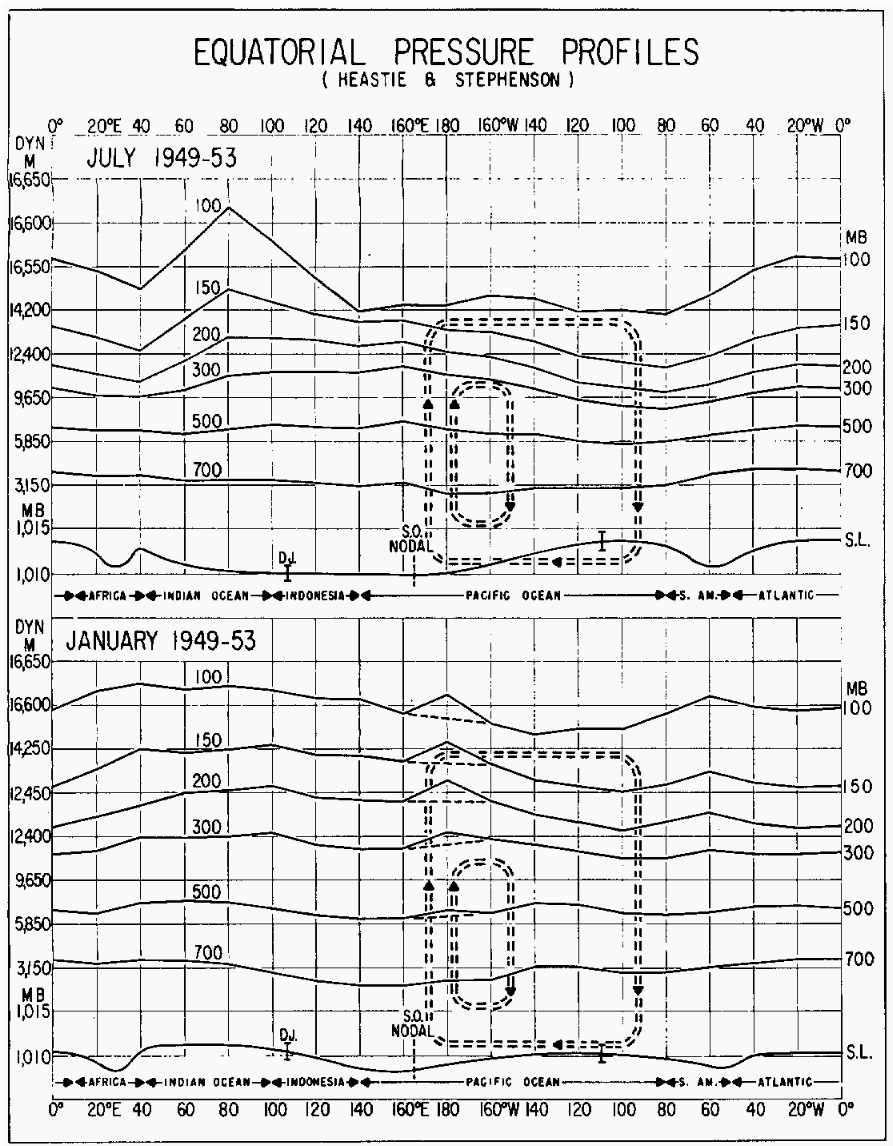
\includegraphics[width=0.9\linewidth]{figures/equatorial-pressure-profiles.png}
  \caption{Height of isobaric streamlines along equator. The \emph{Walker
      circulation} is shown over the Pacific ocean in double-dashed lines, with
    direction indicated by arrows. Source: \citet{bjerknes1969}}
  \label{fig:pressureprofiles}
\end{figure}

Bjerknes states that ``The Walker Circulation ... must be part of the mechanism
of the still larger ``Southern Oscillation'' ...''.

% Diagram here.

%% \cite{bjerknes1969} proposed the currently accepted model for
%% atmospheric circulation driving the SO, calling it the Walker circulation. In
%% this model, dry air sinks over the cool water of the eastern tropical
%% Pacific. After sinking it is transported westward along the equator by the
%% easterly trade winds. As it travels over progressively warmer water the air is
%% warmed and moistened, until it finally reaches the western tropical
%% Pacific. Here the air is now very warm and saturated with water, and it rises in
%% prodigious rain clouds. The circulation is completed with the return flow of air
%% through the upper trophosphere.

%%  % TODO Definitely need some figures here for the Walker circulation.

%% This atmospheric circulation also drives oceanic currents. Water is driven east
%% to west, warming as it goes. This allows for cooler water to rise from the
%% depths along the eastern Pacific, a process called \emph{upwelling}. Combining
%% the oceanic and atmospheric circulations in the Pacific yields a potential
%% explanation for the \elnino\ phenomenon.

\subsection{\elnino-Southern Oscillation}
The Walker circulation requires an east-west tropical Pacific SST gradient for
the transportation of air. An initial positive SST anomaly in the eastern
Pacific ocean would diminish the east-west gradient. A diminished SST gradient
reduces the Walker circulation, in turn weakening the westerly equatorial trade
winds \citep{lindzen1987}. Warm water that was previously being driven westward
by the trade winds can now flow back toward the east, preventing upwelling and
reinforcing the intitial SST anomaly. Through positive feedback between the
ocean and the atmosphere, an initial SST anomaly can lead the equatorial Pacfic
into a warm state -- \elnino. Since the pheneomenon is due to ocean-atmosphere
interaction, the whole system is termed the \elnino-Southern Oscillation
(ENSO). {}\nina\ corresponds to the cold state of ENSO, characterised by
negative SST anomalies and keen trade winds.

%% oscillatory, modes, period

\subsection{Teleconnections}
%take about what drives the teleconnections, i.e. changing circulation
ENSO affects not only the climate of the local Pacific region, but can extend
farther out to influence regions of Africa and Europe \citep{moron1998}. The
magnitude of the influence in these places is weak, but present
nevertheless. Multiple comprehensive studies \citep{ropelewski1987,
  ropelewski1989, nicholson1996} have found that ENSO modulates the rainfall of
continental Africa, although there is some dispute about regional impact
\citep{wolter1989}. Figure \ref{fig:enso_rainfall_anoms} shows the latest
comprehensive study of seasonal rainfall anomalies for ENSO events.

\begin{figure*}
  \centering
  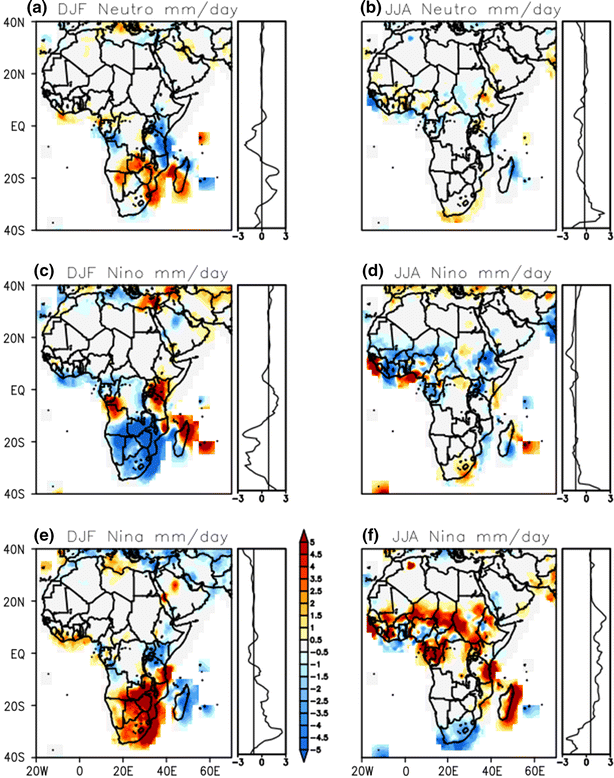
\includegraphics[width=0.7\textwidth]{figures/enso_africa_rainfall_anoms}
  \caption{Distribution of precipitation anomalies and latitudinal averages in
    mm/day, for the DJF and JJA seasons. Panels a) \& b) show neutral years, c)
    \& d) show \elnino\ years and e) \& f) show \nina\ years. The distributions
    show that southern and equatorial Africa exhibit the strongest responses to
    ENSO events, in the DJF and JJA seaons, respectively. DJF corresponds to the
    rainy season and JJA to the dry season for southern Africa and the opposite
    is true for equatorial Africa. Figure taken from \cite{deoliveira2018}.}
  \label{fig:enso_rainfall_anoms}
\end{figure*}

\subsection{Indian Ocean}
On interannual timescales, ENSO is the predominant form of climate variation
\citep{obrien1998}, however it is not the only system that can affect weather on
the African continent. An ocean-atmosphere mode in the Indian Ocean, caused by
anomalously high (low) sea surface temperatures in the western (eastern) regions
of the ocean, was identified by \cite{saji1999} and is starting to be considered
as an influential player in climate dynamics. \cite{anyamba2002} suggest that
the observed vegetation response in regions of Africa between $1997-2000$ was
more significantly driven by these western Indian Ocean SST anomalies, than
anomalies in the Pacific. This mode, called the Indian Ocean Dipole (IOD) has
also been linked to the `Big Dry' -- the severe drought that has been ongoing in
southern Australia since 1995 \citep{karumuri2003, ummenhofer2009}.

Furthermore, the effects of the IOD are not solely continental -- there is
evidence to suggest that the IOD can be involved with the ENSO itself. There
have been multiple studies into its role as a contributor to both the growth
\citep{annamalai2005, hackert2017} and demise \citep{okumura2010, kug2006,
  xie2009, dayan2015} of \elnino{} events. \cite{dong2018} propose that not only
can the IOD influence an established \elnino{} event, but that it may in fact be
able to stop an \elnino{} event developing at all. It follows, then, that in
order to better predict \elnino{} events we must take the Indian Ocean into
account \citep{hackert2017}.

\subsection{Cloud Coverage}
\label{sec:intro:cc}

Fill this out using literature reviews, etc.

\subsection{Normalised Difference Vegetation Index}
\label{sec:intro:ndvi}

Use \cite{yengoh2014}, \cite{bannari1995}, and lit reviews.


% mark you know more about NDVI and calibration so you may want to flesh this
% section out e.g. calibrations
Green vegetation has a distinctive spectral response to electromagnetic
radiation. Radiation in the near-infrared is reflected while the chlorophyll in
leaves absorbs strongly in the red. Hence we determine vegetation coverage using
the normalised difference vegetation index (NDVI) defined as

%% Local Variables:
%% fill-column: 80
%% End:
